\documentclass[12pt,letterpaper,noanswers]{exam}
\usepackage[usenames,dvipsnames,svgnames,table]{xcolor}
\usepackage[margin=0.9in]{geometry}
\renewcommand{\familydefault}{\sfdefault}
\usepackage{multicol}
\pagestyle{head}
\header{AM 111 Class 10}{}{Interpolation, p.\thepage}
\runningheadrule
\headrule
\usepackage{siunitx}
\usepackage{graphicx} % more modern
\usepackage{amsmath} 
\usepackage{amssymb} 
\usepackage{hyperref}
\usepackage{tcolorbox}
\usepackage{enumitem}
\def\mbf{\mathbf}
\newcommand{\vc}[1]{\boldsymbol{#1}}
\def\dsst{\displaystyle}
\DeclareMathOperator*{\argmin}{arg\,min} % thin space, limits underneath in displays


\begin{document}
 \pdfpageheight 11in 
  \pdfpagewidth 8.5in

\noindent 

\section*{Preliminaries}

\begin{itemize}
\itemsep0pt
\item Problem set 04 is due on Friday at noon.
\item There will be a skill check in class during the next class.  The problem info is below.
\item Find all OH on Canvas.
\item Quiz 01 is on Thursday Oct 12.  There is quiz info on canvas.
\end{itemize}



\noindent\textbf{Big picture}

Today: Algorithms for finding a curve that directly passes through data points.

\vspace{0.2cm}
\hrule
\vspace{0.2cm}

\noindent \textbf{Skill check practice}

List the Chebyshev interpolation nodes $x_1, ..., x_n$ on $[-1,1]$ for $n = 3$ ($n$ will be $\leq 5$).


\vspace{0.2cm}
\hrule
\vspace{0.2cm}

\noindent \textbf{Skill check solution}

The nodes are given by $\cos k\pi/(2n)$ for $k$ odd (and $0< k < 2n$).  For $n=3$ we have $\cos \pi/6$, $\cos 3\pi/6$, $\cos 5\pi/6$.



\vspace{0.2cm}
\hrule
\vspace{0.2cm}


\section*{Error when interpolating a polynomial}


\begin{enumerate}
\item Given $n$ points, assume we have an interpolating polynomial $P_{n-1}(t)$.  Add one more point, $(x,f(x))$ to create $P_n(t)$.  Using Newton basis functions, we have $P_n(t) = P_{n-1}(t) + c_n(t-x_1)(t-x_2)...(t-x_n)$ where $P_n(x) = f(x)$.
\begin{parts}
\itemsep60pt
\item Let $h(t) = f(t) - P_{n-1}(t) - c_n(t-x_1)(t-x_2)...(t-x_n)$.  To isolate $c_n$, take the $n$th derivative of your expression.
\item Argue that $h(t) = 0$ at $t = x, x_1, x_2, ..., x_n$. ($n+1$ points)

Rolle's theorem states the following: let $h$ be a continuously differentiable function on the interval $[a,b]$ and assume that $h(a) = h(b)$.  Then there exists a number $c\in (a,b)$ such that $h'(c) = 0$.

\item Using Rolle's theorem, at how many points can you guarantee $h'$ is zero?

\item Using it again, at how many points can you guarantee $h''$ is zero?

\item Argue that there must be one point $c$ for which $h^{(n)}(c) = 0$ (where $c$ is between the smallest and largest of $x, x_1, x_2, ..., x_n$).

\item Substitute $c$ into your expression from part (a) to find $c_n = \frac{1}{n!}f^{(n)}(c)$.
\end{parts}

\end{enumerate}

\vspace{1in}
\subsection*{Runge phenomenon}

For evenly spaced $x_i$ the interpolation error has a characteristic `wiggle' called Runge phenomenon.

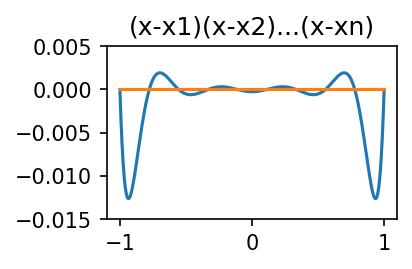
\includegraphics{AM111-F23-CourseNotes/img/C10-error.png}



\section*{Choosing the $x_k$ to minimize error}




\begin{enumerate}[resume]
\itemsep60pt
\item The minimum is achieved by $(x-x_1)...(x-x_n) = \dfrac{1}{2^{n-1}}T_n(x)$ where $T_n(x)$ denotes the degree $n$ Chebyshev polynomial. 
Convince yourself that the $x_i$ are roots of $T_n(x)$.
\item Based on the plots below (one of which shows the evenly spaced case, and the other the Chebyshev spacing), how do the $x_i$ appear to be spaced in the Chebyshev case?

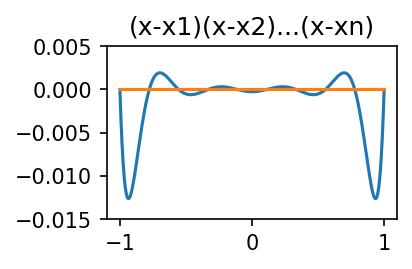
\includegraphics{AM111-F23-CourseNotes/img/C10-error.png}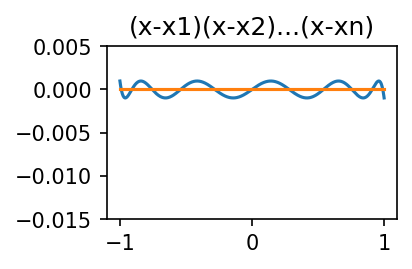
\includegraphics{AM111-F23-CourseNotes/img/C10-error-Ch.png}

\item Consider $f(x) = e^x$ on the interval $[-1,1]$.  Interpolate using $5$ points.

The interpolation error is $\dfrac{f^{(n)}(c)}{n!}(x-x_1)(x-x_2)...(x-x_5)$
\begin{parts}
\itemsep60pt
    \item Find an upper bound for $f^{(5)}(x)$ on this interval.
    \item According to the Chebyshev theorem, $\vert (x-x_1)...(x-x_n)\vert \leq 1/2^{n-1}$.  Assuming five Chebyshev points, write a bound on the maximum value of $\vert (x-x_1)...(x-x_n)\vert$
    \item Write an expression for an upper bound on the interpolation error if using Chebyshev roots for the $x_i$.
\end{parts}
\vspace{1in}
\end{enumerate}
\subsection*{What are the Chebyshev roots?}
The $n$th Chebyshev polynomial is given by $T_n(x) = \cos(n\arccos x)$.

\begin{enumerate}[resume]
\itemsep60pt
\item Find $T_0(x)$.
\item Find $T_1(x)$.
\item Let $y = \arccos x$ so that $\cos y = x$.  Write $T_2(x)$ in terms of $y$.

Use cosine identities to rewrite $T_2(x)$ in terms of $\cos y$ and find $T_2(x)$.
\end{enumerate}

\vspace{1in}

\begin{enumerate}[resume]
\item $T_{n+1}(x) + T_{n-1}(x) = 2\cos(ny)\cos y$ where $\cos ny = T_n(x)$ and $\cos y = x$.  Write a recursion relation for $T_{n+1}(x)$ in terms of $T_n$ and $T_{n-1}$.
\end{enumerate}
\vspace{1in}

Where are the roots of a Chebyshev polynomial?
\begin{enumerate}[resume]
\item Zeros are solutions of $0 = \cos(n\arccos x)$, so $n\arccos x = k\pi/2$ where $k$ is an odd integer.  
\begin{parts}
\itemsep60pt
    \item Rearrange to find $x$.
    \item for $n = 4$ identify the roots.
\end{parts}
\end{enumerate}

\vspace{1in}

\begin{enumerate}[resume]
\item Consider the following four interpolated polynomials fitting $e^{-(4x)^2}$.

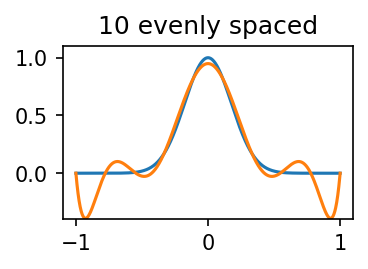
\includegraphics{AM111-F23-CourseNotes/img/C10-gaussian10.png}
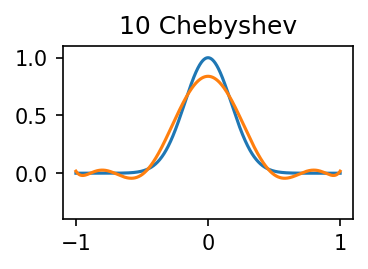
\includegraphics{AM111-F23-CourseNotes/img/C10-gaussian10Ch.png}

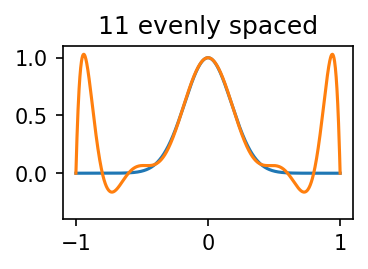
\includegraphics{AM111-F23-CourseNotes/img/C10-gaussian11.png}
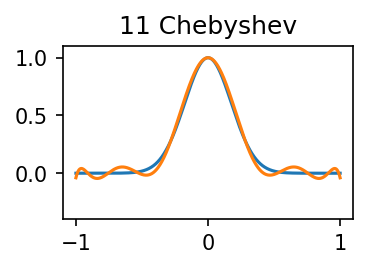
\includegraphics{AM111-F23-CourseNotes/img/C10-gaussian11Ch.png}

Match each to an error curve below:

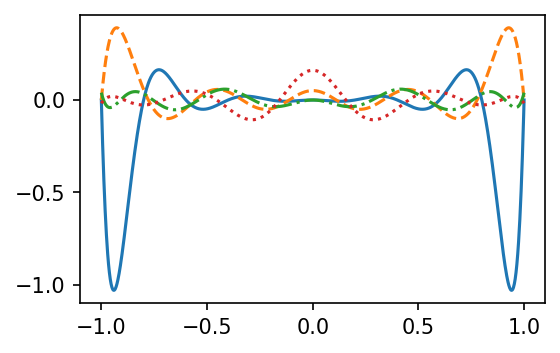
\includegraphics{AM111-F23-CourseNotes/img/C10-gaussianerror.png}

\end{enumerate}

\end{document}